\chapter{Tests}
\label{chap:tests}
In this work, the Context Broker was implemented. A Broker management interface was created, it is shown in Figure \ref{fig:broker}. For testing this implementation, both a Provider and a Consumer interfaces were created, respectively illustrated on Figure \ref{fig:provider} and Figure \ref{fig:consumer}.

The Broker management interface allows a system manager to see the Providers registered in the Broker, shown in Figure \ref{fig:providers}, as well as the context information they have updated to it (Figure \ref{fig:registries}). The manager also has access to the Subscriptions made by Consumers and the \textbf{log} of the Broker system, both shown on Figure \ref{fig:subscriptions} and Figure \ref{fig:log}. The figures also illustrate the results of single operations on each interface of the Broker, using the shown Provider and Consumer interfaces. This is for demonstration of the correct functioning of the Broker: a Provider is registered, makes an update and a Consumer makes a subscription and queries the Broker for information the Provider had inserted. These data can be seen on the Providers, Subscriptions and Registry Table web interfaces of the Broker.


The tests performed were simple, regarding only the correct functionality of the Context Broker. The tests should confirm that the Broker operates correctly, without major response delays, and for a considerate amount of time without errors. The correct operation of a Broker consists on it storing and providing Context Data as it is demanded, given well-formed messages from Consumers and Providers.

For the tests, two Context Providers were created, periodically providing location context data, and two Consumers were created, querying the Broker and subscribing for data as well.

The tests results were successful. They were performed on a computer with a Intel(R) Core(TM) i7-3517U CPU @ 1.90GHz processor, 4GB of memory and Fedora release 20 Linux operating system. The Broker was able to manage the requests and the data without major delays, with an average response time of 80ms. 

\begin{figure}[h]
	\centering
	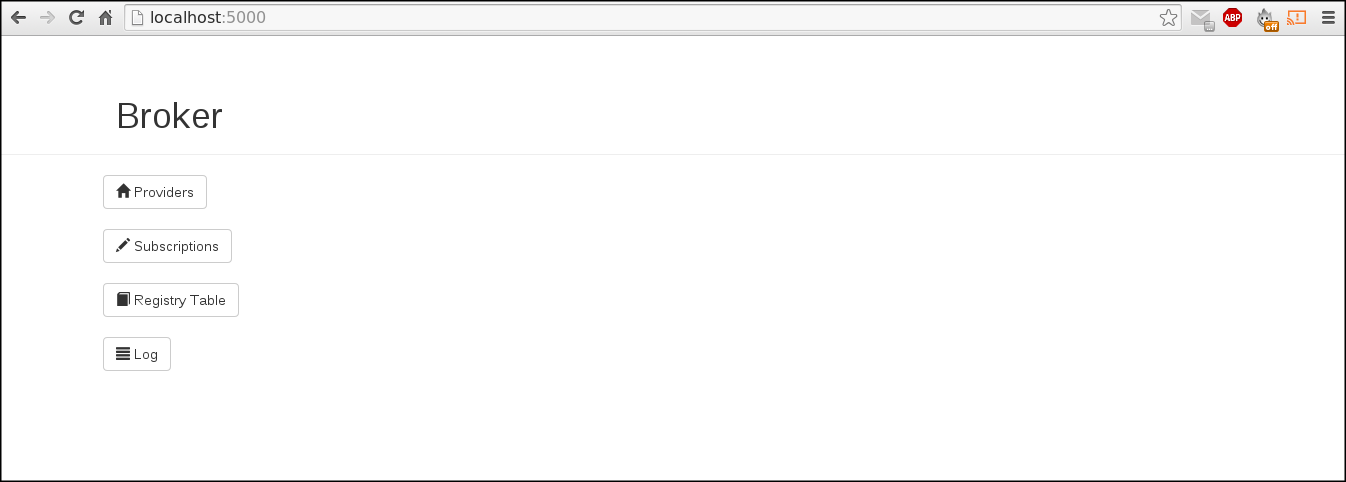
\includegraphics[scale=0.3]{broker.png}
	\caption{Broker Interface}
	\label{fig:broker}
	
\end{figure}

\begin{figure}[h]
	\centering
	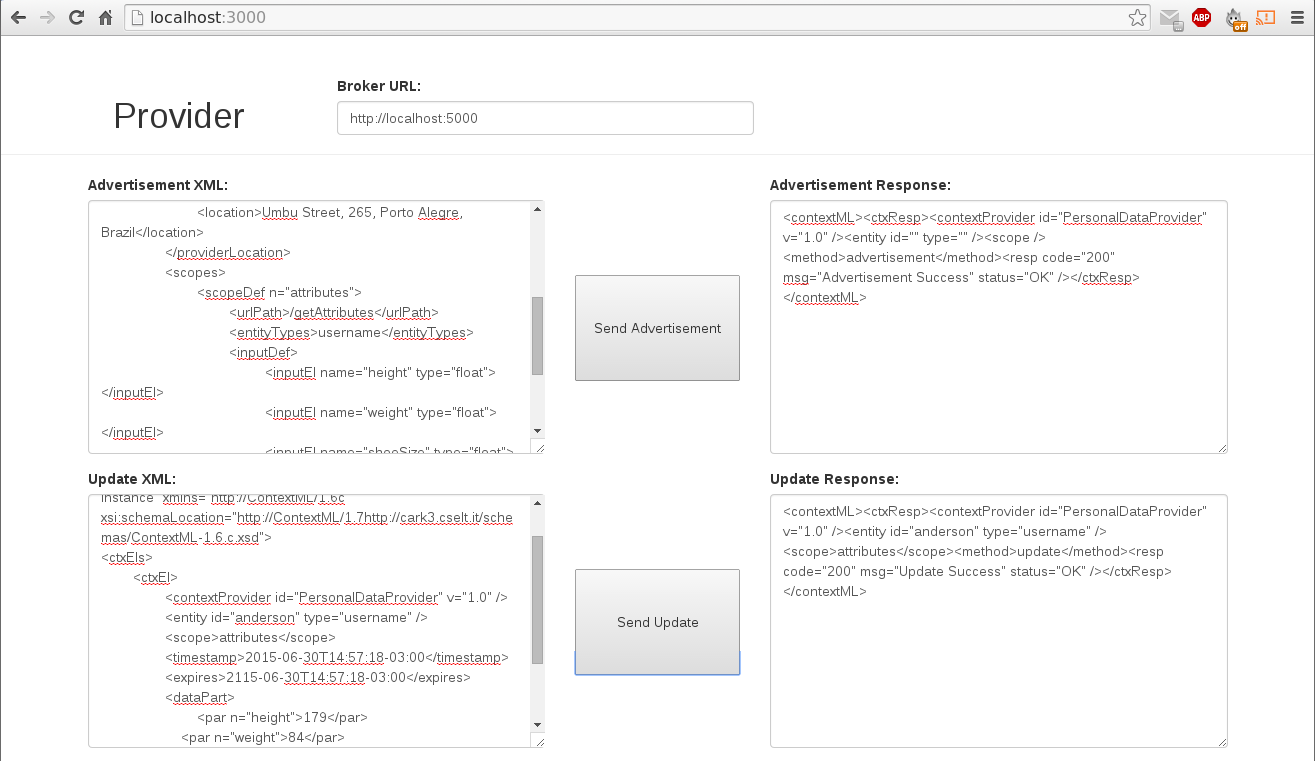
\includegraphics[scale=0.3]{provider.png}
	\caption{Provider Interface}
	\label{fig:provider}
	
\end{figure}

\begin{figure}[h]
	\centering
	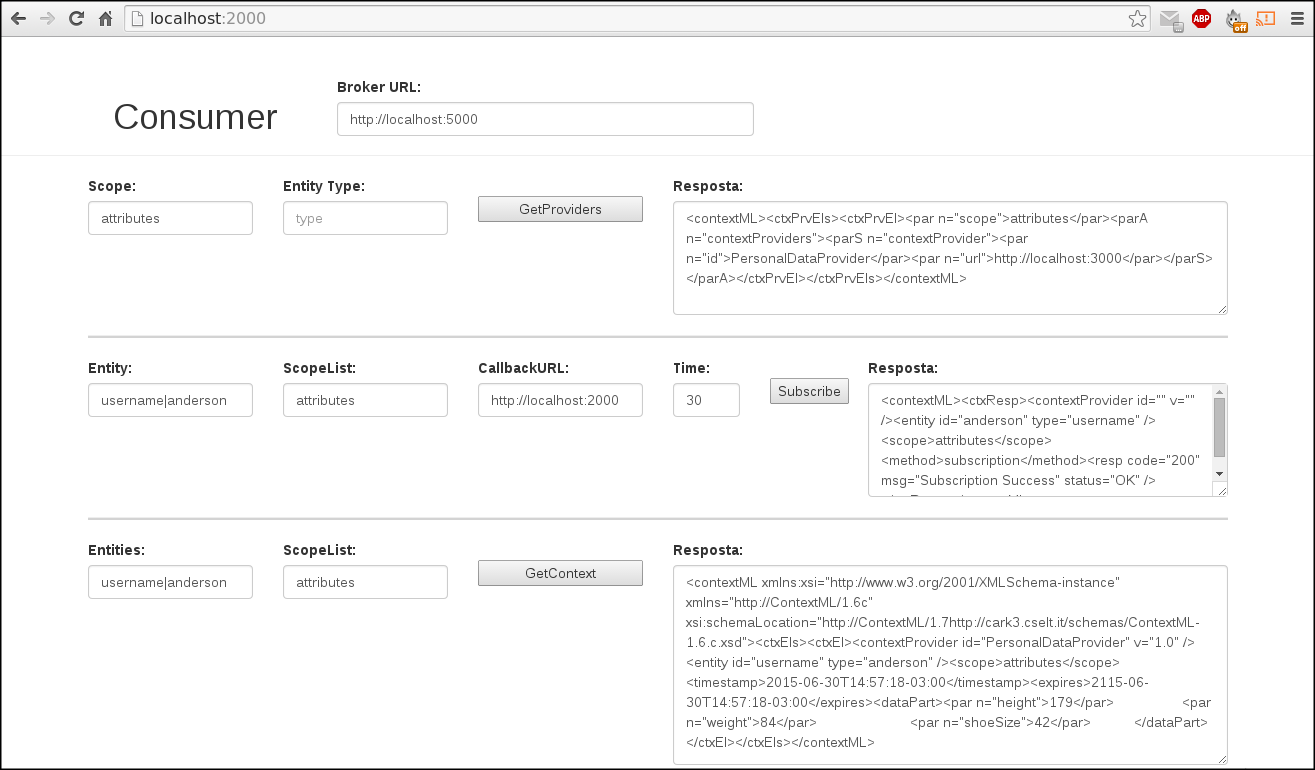
\includegraphics[scale=0.3]{consumer.png}
	\caption{Consumer Interface}
	\label{fig:consumer}
	
\end{figure}

\begin{figure}[h]
	\centering
	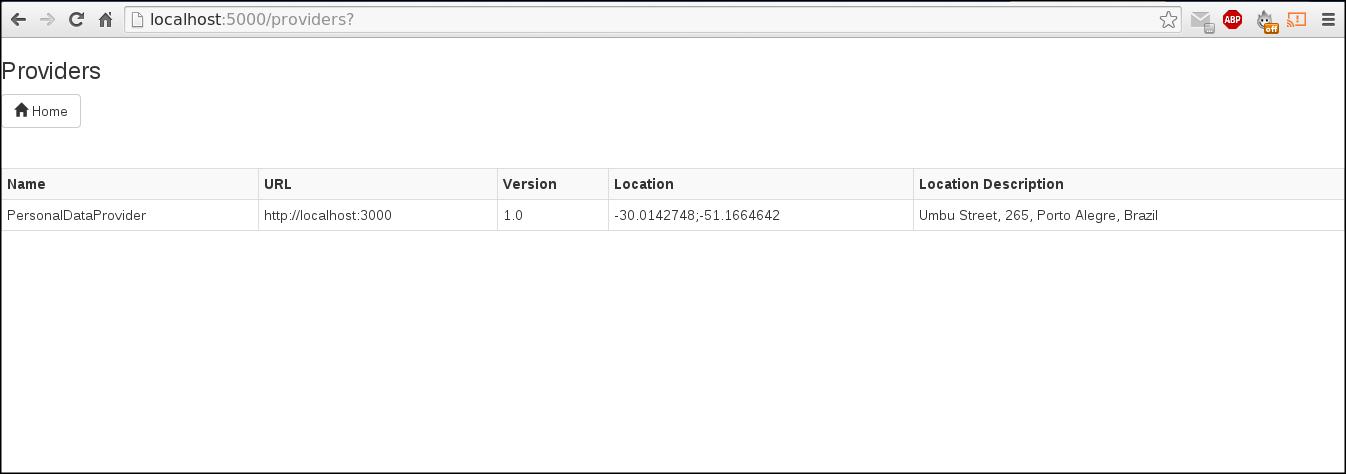
\includegraphics[scale=0.3]{brokerprovs.png}
	\caption{Providers Table}
	\label{fig:brokerprovs}
	
\end{figure}

\begin{figure}[h]
	\centering
	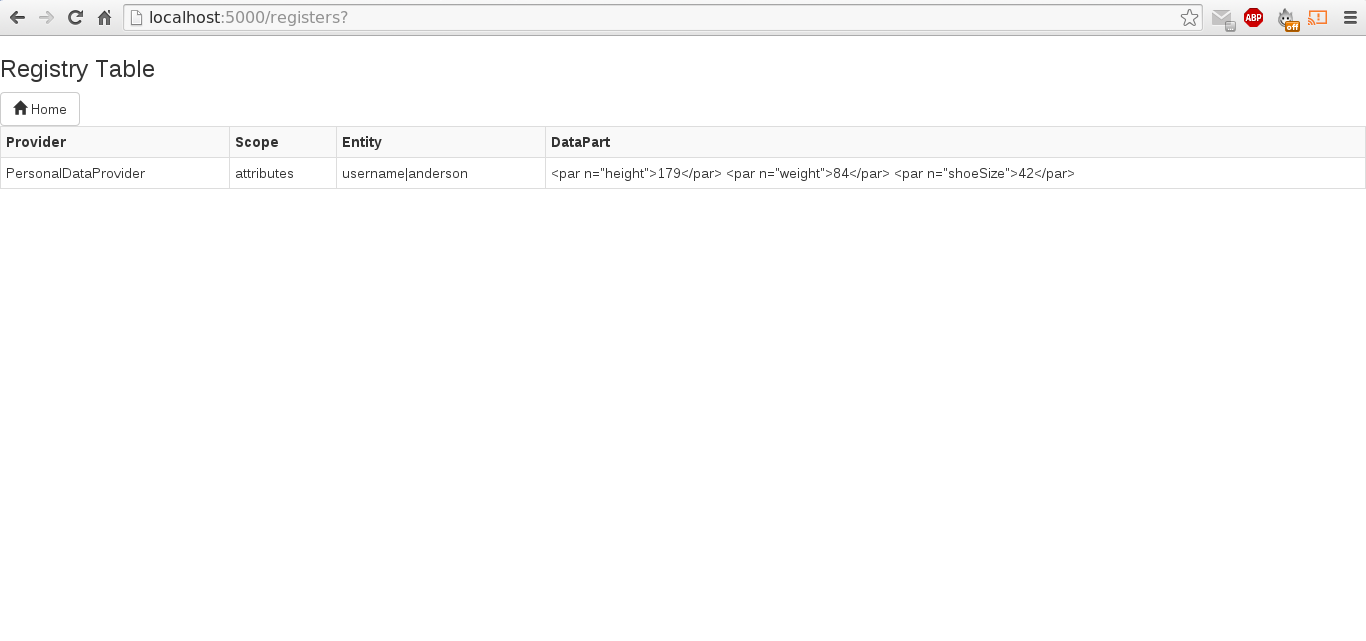
\includegraphics[scale=0.3]{registries.png}
	\caption{Registry Table - Context Information}
	\label{fig:registries}
	
\end{figure}

\begin{figure}[h]
	\centering
	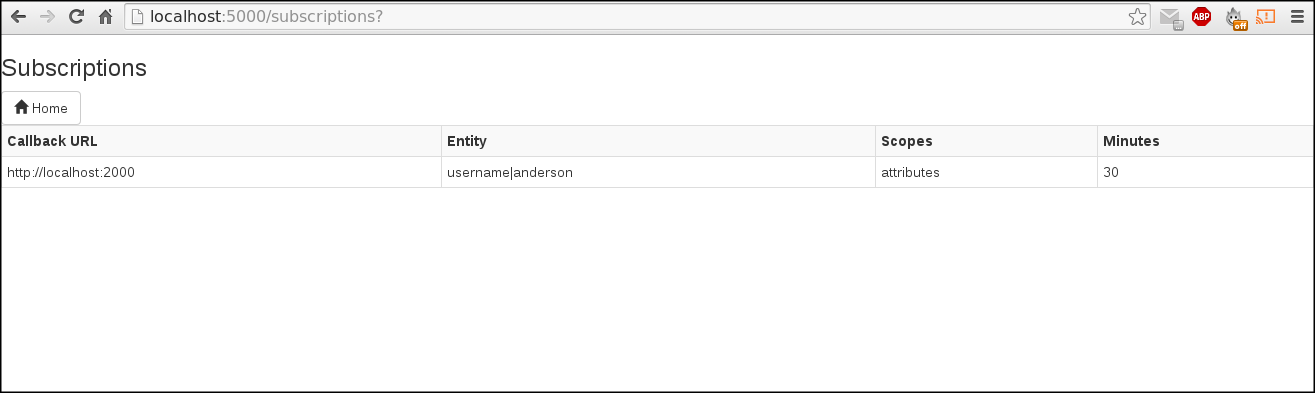
\includegraphics[scale=0.3]{subscriptions.png}
	\caption{Subscriptions Table}
	\label{fig:subscriptions}
	
\end{figure}

\begin{figure}[h]
	\centering
	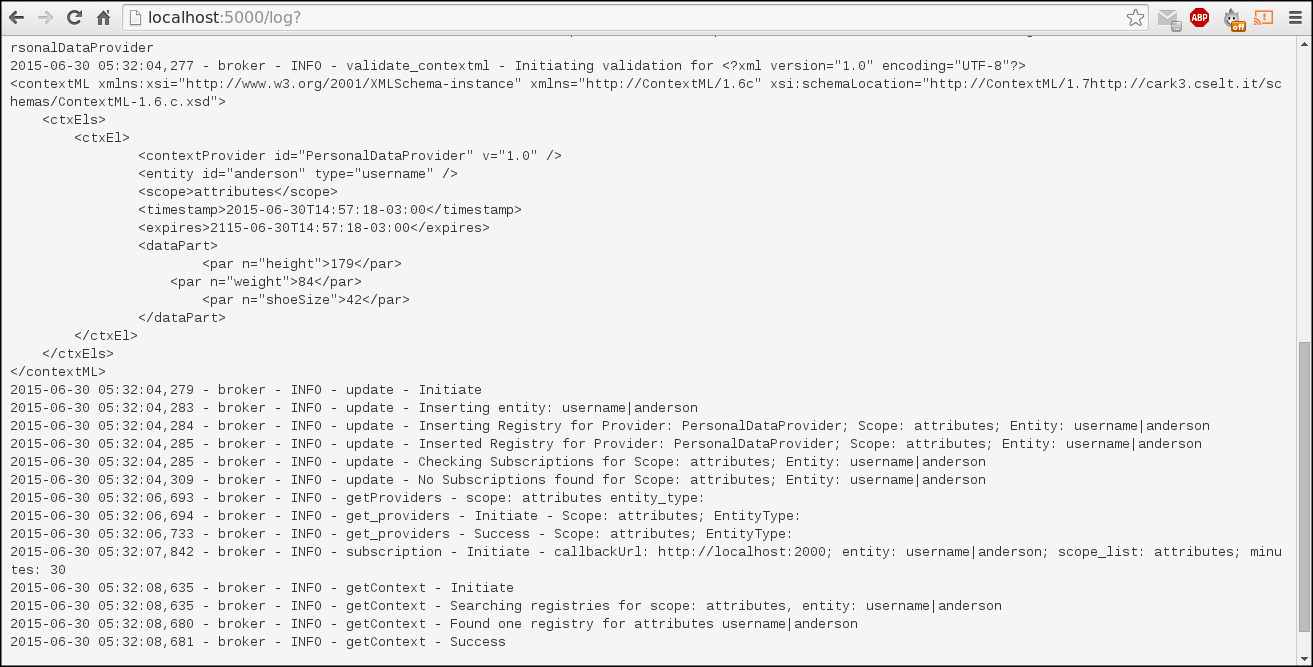
\includegraphics[scale=0.3]{log.png}
	\caption{Broker Log}
	\label{fig:log}
	
\end{figure}

%\todo{perform tests on separate machines, one day execution, create a graph }